
% Default to the notebook output style

    


% Inherit from the specified cell style.




    
\documentclass[11pt]{article}

    
    
    \usepackage[T1]{fontenc}
    % Nicer default font (+ math font) than Computer Modern for most use cases
    \usepackage{mathpazo}

    % Basic figure setup, for now with no caption control since it's done
    % automatically by Pandoc (which extracts ![](path) syntax from Markdown).
    \usepackage{graphicx}
    % We will generate all images so they have a width \maxwidth. This means
    % that they will get their normal width if they fit onto the page, but
    % are scaled down if they would overflow the margins.
    \makeatletter
    \def\maxwidth{\ifdim\Gin@nat@width>\linewidth\linewidth
    \else\Gin@nat@width\fi}
    \makeatother
    \let\Oldincludegraphics\includegraphics
    % Set max figure width to be 80% of text width, for now hardcoded.
    \renewcommand{\includegraphics}[1]{\Oldincludegraphics[width=.8\maxwidth]{#1}}
    % Ensure that by default, figures have no caption (until we provide a
    % proper Figure object with a Caption API and a way to capture that
    % in the conversion process - todo).
    \usepackage{caption}
    \DeclareCaptionLabelFormat{nolabel}{}
    \captionsetup{labelformat=nolabel}

    \usepackage{adjustbox} % Used to constrain images to a maximum size 
    \usepackage{xcolor} % Allow colors to be defined
    \usepackage{enumerate} % Needed for markdown enumerations to work
    \usepackage{geometry} % Used to adjust the document margins
    \usepackage{amsmath} % Equations
    \usepackage{amssymb} % Equations
    \usepackage{textcomp} % defines textquotesingle
    % Hack from http://tex.stackexchange.com/a/47451/13684:
    \AtBeginDocument{%
        \def\PYZsq{\textquotesingle}% Upright quotes in Pygmentized code
    }
    \usepackage{upquote} % Upright quotes for verbatim code
    \usepackage{eurosym} % defines \euro
    \usepackage[mathletters]{ucs} % Extended unicode (utf-8) support
    \usepackage[utf8x]{inputenc} % Allow utf-8 characters in the tex document
    \usepackage{fancyvrb} % verbatim replacement that allows latex
    \usepackage{grffile} % extends the file name processing of package graphics 
                         % to support a larger range 
    % The hyperref package gives us a pdf with properly built
    % internal navigation ('pdf bookmarks' for the table of contents,
    % internal cross-reference links, web links for URLs, etc.)
    \usepackage{hyperref}
    \usepackage{longtable} % longtable support required by pandoc >1.10
    \usepackage{booktabs}  % table support for pandoc > 1.12.2
    \usepackage[inline]{enumitem} % IRkernel/repr support (it uses the enumerate* environment)
    \usepackage[normalem]{ulem} % ulem is needed to support strikethroughs (\sout)
                                % normalem makes italics be italics, not underlines
    

    
    
    % Colors for the hyperref package
    \definecolor{urlcolor}{rgb}{0,.145,.698}
    \definecolor{linkcolor}{rgb}{.71,0.21,0.01}
    \definecolor{citecolor}{rgb}{.12,.54,.11}

    % ANSI colors
    \definecolor{ansi-black}{HTML}{3E424D}
    \definecolor{ansi-black-intense}{HTML}{282C36}
    \definecolor{ansi-red}{HTML}{E75C58}
    \definecolor{ansi-red-intense}{HTML}{B22B31}
    \definecolor{ansi-green}{HTML}{00A250}
    \definecolor{ansi-green-intense}{HTML}{007427}
    \definecolor{ansi-yellow}{HTML}{DDB62B}
    \definecolor{ansi-yellow-intense}{HTML}{B27D12}
    \definecolor{ansi-blue}{HTML}{208FFB}
    \definecolor{ansi-blue-intense}{HTML}{0065CA}
    \definecolor{ansi-magenta}{HTML}{D160C4}
    \definecolor{ansi-magenta-intense}{HTML}{A03196}
    \definecolor{ansi-cyan}{HTML}{60C6C8}
    \definecolor{ansi-cyan-intense}{HTML}{258F8F}
    \definecolor{ansi-white}{HTML}{C5C1B4}
    \definecolor{ansi-white-intense}{HTML}{A1A6B2}

    % commands and environments needed by pandoc snippets
    % extracted from the output of `pandoc -s`
    \providecommand{\tightlist}{%
      \setlength{\itemsep}{0pt}\setlength{\parskip}{0pt}}
    \DefineVerbatimEnvironment{Highlighting}{Verbatim}{commandchars=\\\{\}}
    % Add ',fontsize=\small' for more characters per line
    \newenvironment{Shaded}{}{}
    \newcommand{\KeywordTok}[1]{\textcolor[rgb]{0.00,0.44,0.13}{\textbf{{#1}}}}
    \newcommand{\DataTypeTok}[1]{\textcolor[rgb]{0.56,0.13,0.00}{{#1}}}
    \newcommand{\DecValTok}[1]{\textcolor[rgb]{0.25,0.63,0.44}{{#1}}}
    \newcommand{\BaseNTok}[1]{\textcolor[rgb]{0.25,0.63,0.44}{{#1}}}
    \newcommand{\FloatTok}[1]{\textcolor[rgb]{0.25,0.63,0.44}{{#1}}}
    \newcommand{\CharTok}[1]{\textcolor[rgb]{0.25,0.44,0.63}{{#1}}}
    \newcommand{\StringTok}[1]{\textcolor[rgb]{0.25,0.44,0.63}{{#1}}}
    \newcommand{\CommentTok}[1]{\textcolor[rgb]{0.38,0.63,0.69}{\textit{{#1}}}}
    \newcommand{\OtherTok}[1]{\textcolor[rgb]{0.00,0.44,0.13}{{#1}}}
    \newcommand{\AlertTok}[1]{\textcolor[rgb]{1.00,0.00,0.00}{\textbf{{#1}}}}
    \newcommand{\FunctionTok}[1]{\textcolor[rgb]{0.02,0.16,0.49}{{#1}}}
    \newcommand{\RegionMarkerTok}[1]{{#1}}
    \newcommand{\ErrorTok}[1]{\textcolor[rgb]{1.00,0.00,0.00}{\textbf{{#1}}}}
    \newcommand{\NormalTok}[1]{{#1}}
    
    % Additional commands for more recent versions of Pandoc
    \newcommand{\ConstantTok}[1]{\textcolor[rgb]{0.53,0.00,0.00}{{#1}}}
    \newcommand{\SpecialCharTok}[1]{\textcolor[rgb]{0.25,0.44,0.63}{{#1}}}
    \newcommand{\VerbatimStringTok}[1]{\textcolor[rgb]{0.25,0.44,0.63}{{#1}}}
    \newcommand{\SpecialStringTok}[1]{\textcolor[rgb]{0.73,0.40,0.53}{{#1}}}
    \newcommand{\ImportTok}[1]{{#1}}
    \newcommand{\DocumentationTok}[1]{\textcolor[rgb]{0.73,0.13,0.13}{\textit{{#1}}}}
    \newcommand{\AnnotationTok}[1]{\textcolor[rgb]{0.38,0.63,0.69}{\textbf{\textit{{#1}}}}}
    \newcommand{\CommentVarTok}[1]{\textcolor[rgb]{0.38,0.63,0.69}{\textbf{\textit{{#1}}}}}
    \newcommand{\VariableTok}[1]{\textcolor[rgb]{0.10,0.09,0.49}{{#1}}}
    \newcommand{\ControlFlowTok}[1]{\textcolor[rgb]{0.00,0.44,0.13}{\textbf{{#1}}}}
    \newcommand{\OperatorTok}[1]{\textcolor[rgb]{0.40,0.40,0.40}{{#1}}}
    \newcommand{\BuiltInTok}[1]{{#1}}
    \newcommand{\ExtensionTok}[1]{{#1}}
    \newcommand{\PreprocessorTok}[1]{\textcolor[rgb]{0.74,0.48,0.00}{{#1}}}
    \newcommand{\AttributeTok}[1]{\textcolor[rgb]{0.49,0.56,0.16}{{#1}}}
    \newcommand{\InformationTok}[1]{\textcolor[rgb]{0.38,0.63,0.69}{\textbf{\textit{{#1}}}}}
    \newcommand{\WarningTok}[1]{\textcolor[rgb]{0.38,0.63,0.69}{\textbf{\textit{{#1}}}}}
    
    
    % Define a nice break command that doesn't care if a line doesn't already
    % exist.
    \def\br{\hspace*{\fill} \\* }
    % Math Jax compatability definitions
    \def\gt{>}
    \def\lt{<}
    % Document parameters
    \title{pkpd-tutorial}
    
    
    

    % Pygments definitions
    
\makeatletter
\def\PY@reset{\let\PY@it=\relax \let\PY@bf=\relax%
    \let\PY@ul=\relax \let\PY@tc=\relax%
    \let\PY@bc=\relax \let\PY@ff=\relax}
\def\PY@tok#1{\csname PY@tok@#1\endcsname}
\def\PY@toks#1+{\ifx\relax#1\empty\else%
    \PY@tok{#1}\expandafter\PY@toks\fi}
\def\PY@do#1{\PY@bc{\PY@tc{\PY@ul{%
    \PY@it{\PY@bf{\PY@ff{#1}}}}}}}
\def\PY#1#2{\PY@reset\PY@toks#1+\relax+\PY@do{#2}}

\expandafter\def\csname PY@tok@gh\endcsname{\let\PY@bf=\textbf\def\PY@tc##1{\textcolor[rgb]{0.00,0.00,0.50}{##1}}}
\expandafter\def\csname PY@tok@nf\endcsname{\def\PY@tc##1{\textcolor[rgb]{0.00,0.00,1.00}{##1}}}
\expandafter\def\csname PY@tok@go\endcsname{\def\PY@tc##1{\textcolor[rgb]{0.53,0.53,0.53}{##1}}}
\expandafter\def\csname PY@tok@nl\endcsname{\def\PY@tc##1{\textcolor[rgb]{0.63,0.63,0.00}{##1}}}
\expandafter\def\csname PY@tok@nb\endcsname{\def\PY@tc##1{\textcolor[rgb]{0.00,0.50,0.00}{##1}}}
\expandafter\def\csname PY@tok@kc\endcsname{\let\PY@bf=\textbf\def\PY@tc##1{\textcolor[rgb]{0.00,0.50,0.00}{##1}}}
\expandafter\def\csname PY@tok@no\endcsname{\def\PY@tc##1{\textcolor[rgb]{0.53,0.00,0.00}{##1}}}
\expandafter\def\csname PY@tok@cm\endcsname{\let\PY@it=\textit\def\PY@tc##1{\textcolor[rgb]{0.25,0.50,0.50}{##1}}}
\expandafter\def\csname PY@tok@nn\endcsname{\let\PY@bf=\textbf\def\PY@tc##1{\textcolor[rgb]{0.00,0.00,1.00}{##1}}}
\expandafter\def\csname PY@tok@gd\endcsname{\def\PY@tc##1{\textcolor[rgb]{0.63,0.00,0.00}{##1}}}
\expandafter\def\csname PY@tok@k\endcsname{\let\PY@bf=\textbf\def\PY@tc##1{\textcolor[rgb]{0.00,0.50,0.00}{##1}}}
\expandafter\def\csname PY@tok@m\endcsname{\def\PY@tc##1{\textcolor[rgb]{0.40,0.40,0.40}{##1}}}
\expandafter\def\csname PY@tok@err\endcsname{\def\PY@bc##1{\setlength{\fboxsep}{0pt}\fcolorbox[rgb]{1.00,0.00,0.00}{1,1,1}{\strut ##1}}}
\expandafter\def\csname PY@tok@c1\endcsname{\let\PY@it=\textit\def\PY@tc##1{\textcolor[rgb]{0.25,0.50,0.50}{##1}}}
\expandafter\def\csname PY@tok@bp\endcsname{\def\PY@tc##1{\textcolor[rgb]{0.00,0.50,0.00}{##1}}}
\expandafter\def\csname PY@tok@gu\endcsname{\let\PY@bf=\textbf\def\PY@tc##1{\textcolor[rgb]{0.50,0.00,0.50}{##1}}}
\expandafter\def\csname PY@tok@s1\endcsname{\def\PY@tc##1{\textcolor[rgb]{0.73,0.13,0.13}{##1}}}
\expandafter\def\csname PY@tok@ge\endcsname{\let\PY@it=\textit}
\expandafter\def\csname PY@tok@sc\endcsname{\def\PY@tc##1{\textcolor[rgb]{0.73,0.13,0.13}{##1}}}
\expandafter\def\csname PY@tok@sr\endcsname{\def\PY@tc##1{\textcolor[rgb]{0.73,0.40,0.53}{##1}}}
\expandafter\def\csname PY@tok@mf\endcsname{\def\PY@tc##1{\textcolor[rgb]{0.40,0.40,0.40}{##1}}}
\expandafter\def\csname PY@tok@sd\endcsname{\let\PY@it=\textit\def\PY@tc##1{\textcolor[rgb]{0.73,0.13,0.13}{##1}}}
\expandafter\def\csname PY@tok@mb\endcsname{\def\PY@tc##1{\textcolor[rgb]{0.40,0.40,0.40}{##1}}}
\expandafter\def\csname PY@tok@o\endcsname{\def\PY@tc##1{\textcolor[rgb]{0.40,0.40,0.40}{##1}}}
\expandafter\def\csname PY@tok@mo\endcsname{\def\PY@tc##1{\textcolor[rgb]{0.40,0.40,0.40}{##1}}}
\expandafter\def\csname PY@tok@kd\endcsname{\let\PY@bf=\textbf\def\PY@tc##1{\textcolor[rgb]{0.00,0.50,0.00}{##1}}}
\expandafter\def\csname PY@tok@mi\endcsname{\def\PY@tc##1{\textcolor[rgb]{0.40,0.40,0.40}{##1}}}
\expandafter\def\csname PY@tok@kp\endcsname{\def\PY@tc##1{\textcolor[rgb]{0.00,0.50,0.00}{##1}}}
\expandafter\def\csname PY@tok@s\endcsname{\def\PY@tc##1{\textcolor[rgb]{0.73,0.13,0.13}{##1}}}
\expandafter\def\csname PY@tok@w\endcsname{\def\PY@tc##1{\textcolor[rgb]{0.73,0.73,0.73}{##1}}}
\expandafter\def\csname PY@tok@gi\endcsname{\def\PY@tc##1{\textcolor[rgb]{0.00,0.63,0.00}{##1}}}
\expandafter\def\csname PY@tok@gs\endcsname{\let\PY@bf=\textbf}
\expandafter\def\csname PY@tok@mh\endcsname{\def\PY@tc##1{\textcolor[rgb]{0.40,0.40,0.40}{##1}}}
\expandafter\def\csname PY@tok@vc\endcsname{\def\PY@tc##1{\textcolor[rgb]{0.10,0.09,0.49}{##1}}}
\expandafter\def\csname PY@tok@s2\endcsname{\def\PY@tc##1{\textcolor[rgb]{0.73,0.13,0.13}{##1}}}
\expandafter\def\csname PY@tok@vm\endcsname{\def\PY@tc##1{\textcolor[rgb]{0.10,0.09,0.49}{##1}}}
\expandafter\def\csname PY@tok@nc\endcsname{\let\PY@bf=\textbf\def\PY@tc##1{\textcolor[rgb]{0.00,0.00,1.00}{##1}}}
\expandafter\def\csname PY@tok@gr\endcsname{\def\PY@tc##1{\textcolor[rgb]{1.00,0.00,0.00}{##1}}}
\expandafter\def\csname PY@tok@fm\endcsname{\def\PY@tc##1{\textcolor[rgb]{0.00,0.00,1.00}{##1}}}
\expandafter\def\csname PY@tok@kt\endcsname{\def\PY@tc##1{\textcolor[rgb]{0.69,0.00,0.25}{##1}}}
\expandafter\def\csname PY@tok@cpf\endcsname{\let\PY@it=\textit\def\PY@tc##1{\textcolor[rgb]{0.25,0.50,0.50}{##1}}}
\expandafter\def\csname PY@tok@il\endcsname{\def\PY@tc##1{\textcolor[rgb]{0.40,0.40,0.40}{##1}}}
\expandafter\def\csname PY@tok@nt\endcsname{\let\PY@bf=\textbf\def\PY@tc##1{\textcolor[rgb]{0.00,0.50,0.00}{##1}}}
\expandafter\def\csname PY@tok@kn\endcsname{\let\PY@bf=\textbf\def\PY@tc##1{\textcolor[rgb]{0.00,0.50,0.00}{##1}}}
\expandafter\def\csname PY@tok@se\endcsname{\let\PY@bf=\textbf\def\PY@tc##1{\textcolor[rgb]{0.73,0.40,0.13}{##1}}}
\expandafter\def\csname PY@tok@si\endcsname{\let\PY@bf=\textbf\def\PY@tc##1{\textcolor[rgb]{0.73,0.40,0.53}{##1}}}
\expandafter\def\csname PY@tok@vi\endcsname{\def\PY@tc##1{\textcolor[rgb]{0.10,0.09,0.49}{##1}}}
\expandafter\def\csname PY@tok@sx\endcsname{\def\PY@tc##1{\textcolor[rgb]{0.00,0.50,0.00}{##1}}}
\expandafter\def\csname PY@tok@na\endcsname{\def\PY@tc##1{\textcolor[rgb]{0.49,0.56,0.16}{##1}}}
\expandafter\def\csname PY@tok@cs\endcsname{\let\PY@it=\textit\def\PY@tc##1{\textcolor[rgb]{0.25,0.50,0.50}{##1}}}
\expandafter\def\csname PY@tok@sh\endcsname{\def\PY@tc##1{\textcolor[rgb]{0.73,0.13,0.13}{##1}}}
\expandafter\def\csname PY@tok@vg\endcsname{\def\PY@tc##1{\textcolor[rgb]{0.10,0.09,0.49}{##1}}}
\expandafter\def\csname PY@tok@sa\endcsname{\def\PY@tc##1{\textcolor[rgb]{0.73,0.13,0.13}{##1}}}
\expandafter\def\csname PY@tok@gp\endcsname{\let\PY@bf=\textbf\def\PY@tc##1{\textcolor[rgb]{0.00,0.00,0.50}{##1}}}
\expandafter\def\csname PY@tok@nv\endcsname{\def\PY@tc##1{\textcolor[rgb]{0.10,0.09,0.49}{##1}}}
\expandafter\def\csname PY@tok@nd\endcsname{\def\PY@tc##1{\textcolor[rgb]{0.67,0.13,1.00}{##1}}}
\expandafter\def\csname PY@tok@cp\endcsname{\def\PY@tc##1{\textcolor[rgb]{0.74,0.48,0.00}{##1}}}
\expandafter\def\csname PY@tok@sb\endcsname{\def\PY@tc##1{\textcolor[rgb]{0.73,0.13,0.13}{##1}}}
\expandafter\def\csname PY@tok@ch\endcsname{\let\PY@it=\textit\def\PY@tc##1{\textcolor[rgb]{0.25,0.50,0.50}{##1}}}
\expandafter\def\csname PY@tok@dl\endcsname{\def\PY@tc##1{\textcolor[rgb]{0.73,0.13,0.13}{##1}}}
\expandafter\def\csname PY@tok@ow\endcsname{\let\PY@bf=\textbf\def\PY@tc##1{\textcolor[rgb]{0.67,0.13,1.00}{##1}}}
\expandafter\def\csname PY@tok@gt\endcsname{\def\PY@tc##1{\textcolor[rgb]{0.00,0.27,0.87}{##1}}}
\expandafter\def\csname PY@tok@c\endcsname{\let\PY@it=\textit\def\PY@tc##1{\textcolor[rgb]{0.25,0.50,0.50}{##1}}}
\expandafter\def\csname PY@tok@ni\endcsname{\let\PY@bf=\textbf\def\PY@tc##1{\textcolor[rgb]{0.60,0.60,0.60}{##1}}}
\expandafter\def\csname PY@tok@kr\endcsname{\let\PY@bf=\textbf\def\PY@tc##1{\textcolor[rgb]{0.00,0.50,0.00}{##1}}}
\expandafter\def\csname PY@tok@ss\endcsname{\def\PY@tc##1{\textcolor[rgb]{0.10,0.09,0.49}{##1}}}
\expandafter\def\csname PY@tok@ne\endcsname{\let\PY@bf=\textbf\def\PY@tc##1{\textcolor[rgb]{0.82,0.25,0.23}{##1}}}

\def\PYZbs{\char`\\}
\def\PYZus{\char`\_}
\def\PYZob{\char`\{}
\def\PYZcb{\char`\}}
\def\PYZca{\char`\^}
\def\PYZam{\char`\&}
\def\PYZlt{\char`\<}
\def\PYZgt{\char`\>}
\def\PYZsh{\char`\#}
\def\PYZpc{\char`\%}
\def\PYZdl{\char`\$}
\def\PYZhy{\char`\-}
\def\PYZsq{\char`\'}
\def\PYZdq{\char`\"}
\def\PYZti{\char`\~}
% for compatibility with earlier versions
\def\PYZat{@}
\def\PYZlb{[}
\def\PYZrb{]}
\makeatother


    % Exact colors from NB
    \definecolor{incolor}{rgb}{0.0, 0.0, 0.5}
    \definecolor{outcolor}{rgb}{0.545, 0.0, 0.0}



    
    % Prevent overflowing lines due to hard-to-break entities
    \sloppy 
    % Setup hyperref package
    \hypersetup{
      breaklinks=true,  % so long urls are correctly broken across lines
      colorlinks=true,
      urlcolor=urlcolor,
      linkcolor=linkcolor,
      citecolor=citecolor,
      }
    % Slightly bigger margins than the latex defaults
    
    \geometry{verbose,tmargin=1in,bmargin=1in,lmargin=1in,rmargin=1in}
    
    

    \begin{document}
    
    
    \maketitle
    
    

    
    \section{pbpk-tutorial}\label{pbpk-tutorial}

\subsection{Whole-body physiological based pharmacokinetics model for
caffeine}\label{whole-body-physiological-based-pharmacokinetics-model-for-caffeine}

The model describes clearance of caffeine by the liver in Humans.

\begin{itemize}
\tightlist
\item
  Caffeine and the primary metabolite paraxanthine are removed from the
  blood stream by hepatic or renal clearance.
\item
  Caffeine can be applied either as intra-venous injection or by oral
  dose in the model
\end{itemize}

This notebook demonstrates some simple use cases and analysis of the
model.

\begin{itemize}
\tightlist
\item
  the ODE equations were generate directly from the SBML of the caffeine
  model
\item
  initial values \texttt{X0}, parameter values \texttt{pars}, and the
  ODE system \texttt{dxdt} are defined in the \texttt{caffeine.py}
\end{itemize}

\begin{figure}[htbp]
\centering
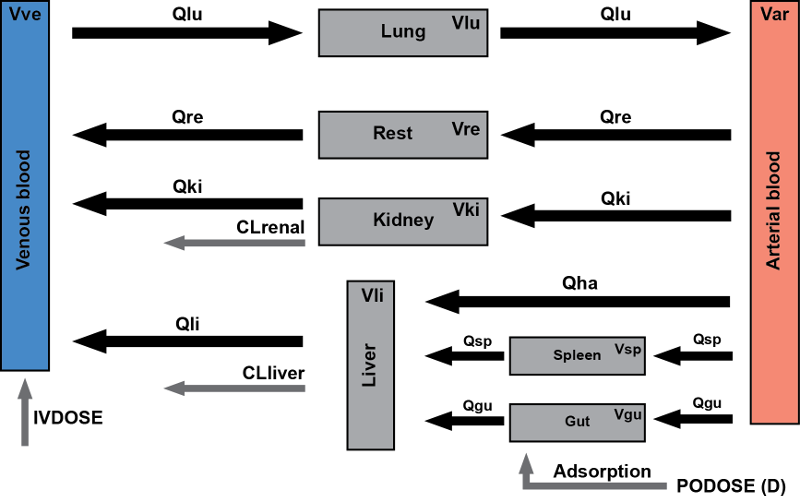
\includegraphics{figures/caffeine_pkpd.png}
\caption{Fig.1 Caffeine PKPD Model}
\end{figure}

This tutorial works in a minimal python environment with the following
package

\begin{verbatim}
numpy
scipy
matplotlib
pandas
libroadrunner
\end{verbatim}

The packages can be installed via

\begin{verbatim}
pip install numpy scipy matplotlib pandas libroadrunner
\end{verbatim}

or in \texttt{conda} via

\begin{verbatim}
pip install numpy scipy matplotlib pandas libroadrunner
\end{verbatim}

For questions contact konigmatt@googlemail.com. The latest version of
the resources are available from
https://github.com/matthiaskoenig/pkpd-tutorial with

\begin{itemize}
\tightlist
\item
  \href{https://github.com/matthiaskoenig/pkpd-tutorial/blob/master/notebooks/caffeine.py}{notebooks/caffeine.py}
\item
  \href{https://github.com/matthiaskoenig/pkpd-tutorial/blob/master/notebooks/pkpd-tutorial.ipynb}{notebooks/pkpd-tutorial.ipynb}
\end{itemize}

    \begin{Verbatim}[commandchars=\\\{\}]
{\color{incolor}In [{\color{incolor}1}]:} \PY{c+c1}{\PYZsh{} general imports for ode integration}
        \PY{k+kn}{import} \PY{n+nn}{numpy} \PY{k+kn}{as} \PY{n+nn}{np}
        \PY{k+kn}{import} \PY{n+nn}{pandas} \PY{k+kn}{as} \PY{n+nn}{pd}
        \PY{k+kn}{import} \PY{n+nn}{roadrunner}
        \PY{k+kn}{from} \PY{n+nn}{matplotlib} \PY{k+kn}{import} \PY{n}{pylab} \PY{k}{as} \PY{n}{plt}
        \PY{k+kn}{from} \PY{n+nn}{pprint} \PY{k+kn}{import} \PY{n}{pprint}
        \PY{k+kn}{from} \PY{n+nn}{helpers} \PY{k+kn}{import} \PY{o}{*}
        
        \PY{c+c1}{\PYZsh{} global settings for plots (optional)}
        \PY{n}{plt}\PY{o}{.}\PY{n}{rcParams}\PY{o}{.}\PY{n}{update}\PY{p}{(}\PY{p}{\PYZob{}}
                \PY{l+s+s1}{\PYZsq{}}\PY{l+s+s1}{axes.labelsize}\PY{l+s+s1}{\PYZsq{}}\PY{p}{:} \PY{l+s+s1}{\PYZsq{}}\PY{l+s+s1}{large}\PY{l+s+s1}{\PYZsq{}}\PY{p}{,} 
                \PY{l+s+s1}{\PYZsq{}}\PY{l+s+s1}{axes.labelweight}\PY{l+s+s1}{\PYZsq{}}\PY{p}{:} \PY{l+s+s1}{\PYZsq{}}\PY{l+s+s1}{bold}\PY{l+s+s1}{\PYZsq{}}\PY{p}{,}
                \PY{l+s+s1}{\PYZsq{}}\PY{l+s+s1}{axes.titlesize}\PY{l+s+s1}{\PYZsq{}}\PY{p}{:} \PY{l+s+s1}{\PYZsq{}}\PY{l+s+s1}{large}\PY{l+s+s1}{\PYZsq{}}\PY{p}{,}
                \PY{l+s+s1}{\PYZsq{}}\PY{l+s+s1}{axes.titleweight}\PY{l+s+s1}{\PYZsq{}}\PY{p}{:} \PY{l+s+s1}{\PYZsq{}}\PY{l+s+s1}{bold}\PY{l+s+s1}{\PYZsq{}}\PY{p}{,}
                \PY{l+s+s1}{\PYZsq{}}\PY{l+s+s1}{legend.fontsize}\PY{l+s+s1}{\PYZsq{}}\PY{p}{:} \PY{l+s+s1}{\PYZsq{}}\PY{l+s+s1}{small}\PY{l+s+s1}{\PYZsq{}}\PY{p}{,}
                \PY{l+s+s1}{\PYZsq{}}\PY{l+s+s1}{xtick.labelsize}\PY{l+s+s1}{\PYZsq{}}\PY{p}{:} \PY{l+s+s1}{\PYZsq{}}\PY{l+s+s1}{large}\PY{l+s+s1}{\PYZsq{}}\PY{p}{,}
                \PY{l+s+s1}{\PYZsq{}}\PY{l+s+s1}{ytick.labelsize}\PY{l+s+s1}{\PYZsq{}}\PY{p}{:} \PY{l+s+s1}{\PYZsq{}}\PY{l+s+s1}{large}\PY{l+s+s1}{\PYZsq{}}\PY{p}{,}
            \PY{p}{\PYZcb{}}\PY{p}{)}
\end{Verbatim}


    \subsection{Load the caffeine model}\label{load-the-caffeine-model}

The full model report with information about the parameter names is
available at

    \begin{Verbatim}[commandchars=\\\{\}]
{\color{incolor}In [{\color{incolor}2}]:} \PY{c+c1}{\PYZsh{} load the model}
        \PY{n}{r} \PY{o}{=} \PY{n}{roadrunner}\PY{o}{.}\PY{n}{RoadRunner}\PY{p}{(}\PY{n}{caffeine\PYZus{}model}\PY{p}{)}
        \PY{c+c1}{\PYZsh{} set variables in result}
        \PY{n}{r}\PY{o}{.}\PY{n}{timeCourseSelections} \PY{o}{=} \PY{p}{[}\PY{l+s+s2}{\PYZdq{}}\PY{l+s+s2}{time}\PY{l+s+s2}{\PYZdq{}}\PY{p}{]} \PY{o}{+} \PY{n}{r}\PY{o}{.}\PY{n}{model}\PY{o}{.}\PY{n}{getFloatingSpeciesIds}\PY{p}{(}\PY{p}{)} \PY{o}{+} \PY{n}{r}\PY{o}{.}\PY{n}{model}\PY{o}{.}\PY{n}{getGlobalParameterIds}\PY{p}{(}\PY{p}{)}
        \PY{c+c1}{\PYZsh{} pprint(r.timeCourseSelections)}
\end{Verbatim}


    \subsection{Example simulation}\label{example-simulation}

We now simulate a 100 {[}mg{]} oral dose (p.o) of caffeine. In a first
step we perform this simulation and look at some state variables of the
model.

The model time is in {[}h{]}. The simulation result is a pandas
DataFrame which can easily be accessed.

    \begin{Verbatim}[commandchars=\\\{\}]
{\color{incolor}In [{\color{incolor}3}]:} \PY{c+c1}{\PYZsh{} reset model to initial state}
        \PY{n}{r}\PY{o}{.}\PY{n}{reset}\PY{p}{(}\PY{n}{roadrunner}\PY{o}{.}\PY{n}{SelectionRecord}\PY{o}{.}\PY{n}{ALL}\PY{p}{)}
        
        \PY{c+c1}{\PYZsh{} set the oral dose}
        \PY{n}{r}\PY{p}{[}\PY{l+s+s1}{\PYZsq{}}\PY{l+s+s1}{init(PODOSE\PYZus{}caf)}\PY{l+s+s1}{\PYZsq{}}\PY{p}{]} \PY{o}{=} \PY{l+m+mi}{100}  \PY{c+c1}{\PYZsh{} [mg]}
        
        \PY{c+c1}{\PYZsh{} simulate the model for 24[h]}
        \PY{n}{s} \PY{o}{=} \PY{n}{simulate}\PY{p}{(}\PY{n}{r}\PY{p}{,} \PY{n}{start}\PY{o}{=}\PY{l+m+mi}{0}\PY{p}{,} \PY{n}{end}\PY{o}{=}\PY{l+m+mi}{24}\PY{p}{,} \PY{n}{steps}\PY{o}{=}\PY{l+m+mi}{500}\PY{p}{)}
        
        \PY{c+c1}{\PYZsh{} show the resulting DataFrame}
        \PY{n}{display}\PY{p}{(}\PY{n}{s}\PY{o}{.}\PY{n}{head}\PY{p}{(}\PY{p}{)}\PY{p}{)}
\end{Verbatim}


    
    \begin{verbatim}
    time    BW      CO    FVre    FVgu    FVki   FVli    FVlu    FVsp    FVve  \
0  0.000  70.0  108.33  0.9049  0.0171  0.0044  0.021  0.0076  0.0026  0.0514   
1  0.048  70.0  108.33  0.9049  0.0171  0.0044  0.021  0.0076  0.0026  0.0514   
2  0.096  70.0  108.33  0.9049  0.0171  0.0044  0.021  0.0076  0.0026  0.0514   
3  0.144  70.0  108.33  0.9049  0.0171  0.0044  0.021  0.0076  0.0026  0.0514   
4  0.192  70.0  108.33  0.9049  0.0171  0.0044  0.021  0.0076  0.0026  0.0514   

     ...     Cli_free_px  Cki_free_px  CLliv_px   vliv_px  Absorption_caf  \
0    ...        0.000000     0.000000    11.907  0.000000      250.000000   
1    ...        0.119169     0.012902    11.907  1.418946      221.730109   
2    ...        0.236954     0.053722    11.907  2.821412      196.656965   
3    ...        0.290249     0.086389    11.907  3.455996      174.419082   
4    ...        0.315503     0.111110    11.907  3.756691      154.695848   

   Venous_caf  Absorption_px  Venous_px  Abody_caf  Abody_px  
0    0.000000            0.0   0.000000   0.000000  0.000000  
1  195.237839            0.0  11.283537  10.936949  0.345689  
2  325.289528            0.0  26.719440  20.042439  1.163572  
3  399.057352            0.0  37.908947  27.878691  2.069801  
4  452.052947            0.0  46.762611  34.701221  2.962668  

[5 rows x 110 columns]
    \end{verbatim}

    
    \begin{Verbatim}[commandchars=\\\{\}]
{\color{incolor}In [{\color{incolor}4}]:} \PY{c+c1}{\PYZsh{} plot venous caffeine \PYZam{} paraxanthine against time}
        \PY{n}{f1}\PY{p}{,} \PY{n}{ax1} \PY{o}{=} \PY{n}{plt}\PY{o}{.}\PY{n}{subplots}\PY{p}{(}\PY{l+m+mi}{1}\PY{p}{,} \PY{l+m+mi}{1}\PY{p}{,} \PY{n}{figsize}\PY{o}{=}\PY{p}{(}\PY{l+m+mi}{5}\PY{p}{,} \PY{l+m+mi}{5}\PY{p}{)}\PY{p}{)}
        \PY{n}{ax1}\PY{o}{.}\PY{n}{plot}\PY{p}{(}\PY{n}{s}\PY{o}{.}\PY{n}{time}\PY{p}{,} \PY{n}{s}\PY{o}{.}\PY{n}{Cve\PYZus{}caf}\PY{p}{,} \PY{n}{linewidth}\PY{o}{=}\PY{l+m+mi}{2}\PY{p}{,} \PY{n}{label}\PY{o}{=}\PY{l+s+s2}{\PYZdq{}}\PY{l+s+s2}{caffeine [mg/l]}\PY{l+s+s2}{\PYZdq{}}\PY{p}{)}
        \PY{n}{ax1}\PY{o}{.}\PY{n}{plot}\PY{p}{(}\PY{n}{s}\PY{o}{.}\PY{n}{time}\PY{p}{,} \PY{n}{s}\PY{o}{.}\PY{n}{Cve\PYZus{}px}\PY{p}{,} \PY{n}{linewidth}\PY{o}{=}\PY{l+m+mi}{2}\PY{p}{,} \PY{n}{label}\PY{o}{=}\PY{l+s+s2}{\PYZdq{}}\PY{l+s+s2}{paraxanthine [mg/l]}\PY{l+s+s2}{\PYZdq{}}\PY{p}{)}
        \PY{n}{ax1}\PY{o}{.}\PY{n}{set\PYZus{}title}\PY{p}{(}\PY{l+s+s1}{\PYZsq{}}\PY{l+s+s1}{100 [mg] caffeine (oral dose)}\PY{l+s+s1}{\PYZsq{}}\PY{p}{)}
        \PY{n}{ax1}\PY{o}{.}\PY{n}{set\PYZus{}ylabel}\PY{p}{(}\PY{l+s+s1}{\PYZsq{}}\PY{l+s+s1}{concentration}\PY{l+s+s1}{\PYZsq{}}\PY{p}{)}
        \PY{n}{ax1}\PY{o}{.}\PY{n}{set\PYZus{}xlabel}\PY{p}{(}\PY{l+s+s1}{\PYZsq{}}\PY{l+s+s1}{time [h]}\PY{l+s+s1}{\PYZsq{}}\PY{p}{)}
        \PY{n}{ax1}\PY{o}{.}\PY{n}{legend}\PY{p}{(}\PY{p}{)}
        \PY{n}{plt}\PY{o}{.}\PY{n}{show}\PY{p}{(}\PY{p}{)}
\end{Verbatim}


    \begin{center}
    \adjustimage{max size={0.9\linewidth}{0.9\paperheight}}{output_6_0.png}
    \end{center}
    { \hspace*{\fill} \\}
    
    \subsection{Compare amounts in different
organs}\label{compare-amounts-in-different-organs}

In the following we compare the amount of caffeine in the different
organs. For this we select all the columns in the solution which belong
the amount of caffeine.

    \begin{Verbatim}[commandchars=\\\{\}]
{\color{incolor}In [{\color{incolor}5}]:} \PY{c+c1}{\PYZsh{} plot caffeine and paraxanthine amounts}
        \PY{n}{f1}\PY{p}{,} \PY{n}{ax1} \PY{o}{=} \PY{n}{plt}\PY{o}{.}\PY{n}{subplots}\PY{p}{(}\PY{l+m+mi}{1}\PY{p}{,} \PY{l+m+mi}{1}\PY{p}{,} \PY{n}{figsize}\PY{o}{=}\PY{p}{(}\PY{l+m+mi}{5}\PY{p}{,}\PY{l+m+mi}{5}\PY{p}{)}\PY{p}{)}
        \PY{n}{organs} \PY{o}{=} \PY{p}{[}\PY{l+s+s2}{\PYZdq{}}\PY{l+s+s2}{li}\PY{l+s+s2}{\PYZdq{}}\PY{p}{,} \PY{l+s+s2}{\PYZdq{}}\PY{l+s+s2}{ki}\PY{l+s+s2}{\PYZdq{}}\PY{p}{,} \PY{l+s+s2}{\PYZdq{}}\PY{l+s+s2}{lu}\PY{l+s+s2}{\PYZdq{}}\PY{p}{,} \PY{l+s+s2}{\PYZdq{}}\PY{l+s+s2}{sp}\PY{l+s+s2}{\PYZdq{}}\PY{p}{,} \PY{l+s+s2}{\PYZdq{}}\PY{l+s+s2}{gu}\PY{l+s+s2}{\PYZdq{}}\PY{p}{,} \PY{l+s+s2}{\PYZdq{}}\PY{l+s+s2}{re}\PY{l+s+s2}{\PYZdq{}}\PY{p}{]}
        
        \PY{k}{for} \PY{n}{organ} \PY{o+ow}{in} \PY{n}{organs}\PY{p}{:}
            \PY{n}{sid} \PY{o}{=} \PY{l+s+s2}{\PYZdq{}}\PY{l+s+s2}{A\PYZob{}\PYZcb{}\PYZus{}caf}\PY{l+s+s2}{\PYZdq{}}\PY{o}{.}\PY{n}{format}\PY{p}{(}\PY{n}{organ}\PY{p}{)}
            \PY{n}{label} \PY{o}{=} \PY{l+s+s2}{\PYZdq{}}\PY{l+s+s2}{caffeine (\PYZob{}\PYZcb{}) [mg]}\PY{l+s+s2}{\PYZdq{}}\PY{o}{.}\PY{n}{format}\PY{p}{(}\PY{n}{organ}\PY{p}{)}
            \PY{n}{ax1}\PY{o}{.}\PY{n}{plot}\PY{p}{(}\PY{n}{s}\PY{o}{.}\PY{n}{time}\PY{p}{,} \PY{n}{s}\PY{p}{[}\PY{n}{sid}\PY{p}{]}\PY{p}{,} \PY{n}{label}\PY{o}{=}\PY{n}{label}\PY{p}{)}    
        
        \PY{n}{ax1}\PY{o}{.}\PY{n}{set\PYZus{}ylabel}\PY{p}{(}\PY{l+s+s1}{\PYZsq{}}\PY{l+s+s1}{caffeine [mg]}\PY{l+s+s1}{\PYZsq{}}\PY{p}{)}
        \PY{n}{ax1}\PY{o}{.}\PY{n}{set\PYZus{}xlabel}\PY{p}{(}\PY{l+s+s1}{\PYZsq{}}\PY{l+s+s1}{time [h]}\PY{l+s+s1}{\PYZsq{}}\PY{p}{)}
        \PY{n}{ax1}\PY{o}{.}\PY{n}{legend}\PY{p}{(}\PY{p}{)}
        
        \PY{n}{plt}\PY{o}{.}\PY{n}{show}\PY{p}{(}\PY{p}{)}
\end{Verbatim}


    \begin{center}
    \adjustimage{max size={0.9\linewidth}{0.9\paperheight}}{output_8_0.png}
    \end{center}
    { \hspace*{\fill} \\}
    
    \subsection{Plot the organ volumes}\label{plot-the-organ-volumes}

In the following we plot the organ volumes by querying the model

    \begin{Verbatim}[commandchars=\\\{\}]
{\color{incolor}In [{\color{incolor}6}]:} \PY{k}{for} \PY{n}{oid} \PY{o+ow}{in} \PY{n}{organs}\PY{p}{:}
            \PY{n}{vid} \PY{o}{=} \PY{l+s+s2}{\PYZdq{}}\PY{l+s+s2}{V\PYZob{}\PYZcb{}}\PY{l+s+s2}{\PYZdq{}}\PY{o}{.}\PY{n}{format}\PY{p}{(}\PY{n}{oid}\PY{p}{)}
            \PY{k}{print}\PY{p}{(}\PY{l+s+s2}{\PYZdq{}}\PY{l+s+s2}{V\PYZob{}\PYZcb{} = \PYZob{}\PYZcb{} [l]}\PY{l+s+s2}{\PYZdq{}}\PY{o}{.}\PY{n}{format}\PY{p}{(}\PY{n}{oid}\PY{p}{,} \PY{n}{r}\PY{p}{[}\PY{n}{vid}\PY{p}{]}\PY{p}{)}\PY{p}{)}
\end{Verbatim}


    \begin{Verbatim}[commandchars=\\\{\}]
Vli = 1.47 [l]
Vki = 0.308 [l]
Vlu = 0.532 [l]
Vsp = 0.182 [l]
Vgu = 1.197 [l]
Vre = 63.343 [l]

    \end{Verbatim}

    \subsection{Stepwise increase of the caffeine
dose}\label{stepwise-increase-of-the-caffeine-dose}

Now we see what happens if we drink more coffee every day

    \begin{Verbatim}[commandchars=\\\{\}]
{\color{incolor}In [{\color{incolor}7}]:} \PY{n}{doses} \PY{o}{=} \PY{n}{np}\PY{o}{.}\PY{n}{linspace}\PY{p}{(}\PY{l+m+mi}{0}\PY{p}{,} \PY{l+m+mi}{500}\PY{p}{,} \PY{n}{num}\PY{o}{=}\PY{l+m+mi}{11}\PY{p}{)}
        \PY{n}{results} \PY{o}{=} \PY{p}{[}\PY{p}{]}
        
        \PY{k}{for} \PY{n}{dose} \PY{o+ow}{in} \PY{n}{doses}\PY{p}{:}
            \PY{c+c1}{\PYZsh{} reset model to initial state}
            \PY{n}{r}\PY{o}{.}\PY{n}{reset}\PY{p}{(}\PY{n}{roadrunner}\PY{o}{.}\PY{n}{SelectionRecord}\PY{o}{.}\PY{n}{ALL}\PY{p}{)}
            
            \PY{c+c1}{\PYZsh{} set the oral dose}
            \PY{n}{r}\PY{p}{[}\PY{l+s+s1}{\PYZsq{}}\PY{l+s+s1}{init(PODOSE\PYZus{}caf)}\PY{l+s+s1}{\PYZsq{}}\PY{p}{]} \PY{o}{=} \PY{n}{dose}  \PY{c+c1}{\PYZsh{} [mg]}
        
            \PY{c+c1}{\PYZsh{} simulate the model for 24[h]}
            \PY{n}{s} \PY{o}{=} \PY{n}{simulate}\PY{p}{(}\PY{n}{r}\PY{p}{,} \PY{n}{start}\PY{o}{=}\PY{l+m+mi}{0}\PY{p}{,} \PY{n}{end}\PY{o}{=}\PY{l+m+mi}{24}\PY{p}{,} \PY{n}{steps}\PY{o}{=}\PY{l+m+mi}{500}\PY{p}{)}
            \PY{n}{results}\PY{o}{.}\PY{n}{append}\PY{p}{(}\PY{n}{s}\PY{p}{)}
        
        \PY{c+c1}{\PYZsh{} plot venous caffeine \PYZam{} paraxanthine against time}
        \PY{n}{f1}\PY{p}{,} \PY{n}{ax1} \PY{o}{=} \PY{n}{plt}\PY{o}{.}\PY{n}{subplots}\PY{p}{(}\PY{l+m+mi}{1}\PY{p}{,} \PY{l+m+mi}{1}\PY{p}{,} \PY{n}{figsize}\PY{o}{=}\PY{p}{(}\PY{l+m+mi}{5}\PY{p}{,} \PY{l+m+mi}{5}\PY{p}{)}\PY{p}{)}
        \PY{k}{for} \PY{n}{k}\PY{p}{,} \PY{n}{s} \PY{o+ow}{in} \PY{n+nb}{enumerate}\PY{p}{(}\PY{n}{results}\PY{p}{)}\PY{p}{:}
            \PY{k}{if} \PY{n}{k} \PY{o}{==} \PY{l+m+mi}{1}\PY{p}{:}
                \PY{n}{label} \PY{o}{=} \PY{l+s+s2}{\PYZdq{}}\PY{l+s+s2}{caffeine [mg/l]}\PY{l+s+s2}{\PYZdq{}}
            \PY{k}{else}\PY{p}{:}
                \PY{n}{label} \PY{o}{=} \PY{l+s+s2}{\PYZdq{}}\PY{l+s+s2}{\PYZus{}\PYZus{}nolabel\PYZus{}\PYZus{}}\PY{l+s+s2}{\PYZdq{}}
            \PY{n}{ax1}\PY{o}{.}\PY{n}{plot}\PY{p}{(}\PY{n}{s}\PY{o}{.}\PY{n}{time}\PY{p}{,} \PY{n}{s}\PY{o}{.}\PY{n}{Cve\PYZus{}caf}\PY{p}{,} \PY{n}{linewidth}\PY{o}{=}\PY{l+m+mi}{2}\PY{p}{,} \PY{n}{color}\PY{o}{=}\PY{l+s+s2}{\PYZdq{}}\PY{l+s+s2}{blue}\PY{l+s+s2}{\PYZdq{}}\PY{p}{,} \PY{n}{label}\PY{o}{=}\PY{n}{label}\PY{p}{,} \PY{n}{alpha}\PY{o}{=}\PY{l+m+mf}{0.8}\PY{p}{)}
            \PY{k}{if} \PY{n}{k} \PY{o}{==} \PY{l+m+mi}{1}\PY{p}{:}
                \PY{n}{label} \PY{o}{=} \PY{l+s+s2}{\PYZdq{}}\PY{l+s+s2}{paraxanthine [mg/l]}\PY{l+s+s2}{\PYZdq{}}
            \PY{k}{else}\PY{p}{:}
                \PY{n}{label} \PY{o}{=} \PY{l+s+s2}{\PYZdq{}}\PY{l+s+s2}{\PYZus{}\PYZus{}nolabel\PYZus{}\PYZus{}}\PY{l+s+s2}{\PYZdq{}}
            \PY{n}{ax1}\PY{o}{.}\PY{n}{plot}\PY{p}{(}\PY{n}{s}\PY{o}{.}\PY{n}{time}\PY{p}{,} \PY{n}{s}\PY{o}{.}\PY{n}{Cve\PYZus{}px}\PY{p}{,} \PY{n}{linewidth}\PY{o}{=}\PY{l+m+mi}{2}\PY{p}{,} \PY{n}{color}\PY{o}{=}\PY{l+s+s2}{\PYZdq{}}\PY{l+s+s2}{darkorange}\PY{l+s+s2}{\PYZdq{}}\PY{p}{,} \PY{n}{label}\PY{o}{=}\PY{n}{label}\PY{p}{,} \PY{n}{alpha}\PY{o}{=}\PY{l+m+mf}{0.8}\PY{p}{)}
        \PY{n}{ax1}\PY{o}{.}\PY{n}{set\PYZus{}title}\PY{p}{(}\PY{l+s+s1}{\PYZsq{}}\PY{l+s+s1}{caffeine (oral dose)}\PY{l+s+s1}{\PYZsq{}}\PY{p}{)}
        \PY{n}{ax1}\PY{o}{.}\PY{n}{set\PYZus{}ylabel}\PY{p}{(}\PY{l+s+s1}{\PYZsq{}}\PY{l+s+s1}{concentration}\PY{l+s+s1}{\PYZsq{}}\PY{p}{)}
        \PY{n}{ax1}\PY{o}{.}\PY{n}{set\PYZus{}xlabel}\PY{p}{(}\PY{l+s+s1}{\PYZsq{}}\PY{l+s+s1}{time [h]}\PY{l+s+s1}{\PYZsq{}}\PY{p}{)}
        \PY{n}{ax1}\PY{o}{.}\PY{n}{legend}\PY{p}{(}\PY{p}{)}
        \PY{n}{plt}\PY{o}{.}\PY{n}{show}\PY{p}{(}\PY{p}{)}
\end{Verbatim}


    \begin{center}
    \adjustimage{max size={0.9\linewidth}{0.9\paperheight}}{output_12_0.png}
    \end{center}
    { \hspace*{\fill} \\}
    
    \section{Exercises}\label{exercises}

\subsection{E1 Your caffeine level}\label{e1-your-caffeine-level}

The first exercise is to calculate the timecourse of the expected venous
caffeine level after you drink some caffeinated beverage. To estimate
your oral dose of caffeine you can estimate the caffeine content from
the following chart

\begin{figure}[htbp]
\centering
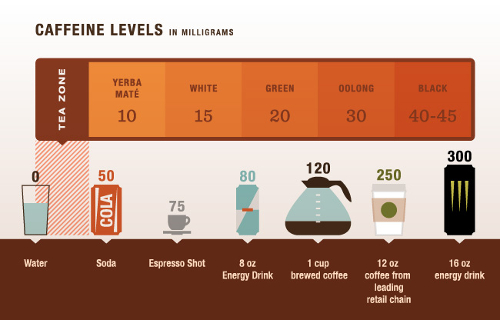
\includegraphics{figures/caffeine_levels.jpg}
\caption{Fig.2 Caffeine Content of Beverages}
\end{figure}

The oral dose is defined in the model via parameter
\texttt{r{[}\textquotesingle{}init(PODOSE\_caf)\textquotesingle{}{]}\ =\ 100}
{[}mg{]}. In addition you can also adjust the bodyweight to get a more
realistic estimation via the parameter
\texttt{r{[}\textquotesingle{}init(BW)\textquotesingle{}{]}\ =\ 70}
{[}kg{]}.

\begin{itemize}
\tightlist
\item
  What would be your level of caffeine now, if you had two cups of
  coffee for breakfast this morning?
\item
  How would your time course and level of caffeine look if you would
  take the same amount of caffeine intravenously (I.V)? (Hint: you have
  to set the set the i.v. dose via
  \texttt{r{[}\textquotesingle{}init(IVDOSE\_caf)\textquotesingle{}{]}\ =\ 100})
\item
  What is the peak time of caffeine in venous blood? What is the peak
  concentration?
\end{itemize}

\subsection{E2 Interindividual
variability}\label{e2-interindividual-variability}

We saw that there is a large variability in caffeine kinetics in the
population. Depending on if you are a fast or slow metabolizer of
caffeine the timecourses can look very different. In E1 you calculated
the mean timecourse for the population. Now we will look at the
interindividual differences.

Your caffeine clearance by the liver depends on the activity of CYP1A2
in the liver, the main enzyme metabolizing caffeine. The activity is
defined via the apparent clearance caffeine by hepatic microsomes
(\texttt{r{[}init(\textquotesingle{}HLM\_CLint\_caf\textquotesingle{}){]}\ =\ 2}
{[}mul/min/mg{]}).

\begin{itemize}
\tightlist
\item
  How would your time course / level of caffeine change if you are a
  slow metabolizer (small apparent clearance), or if you are a fast
  metabolizer (large apperent clearance)?
\item
  Simulate the effect of lifestyle changes on your caffeine clearance
  via adjusting the caffeine clearance accordinly. For instance simulate
  changes in your coffee intake or smoking habit. An overview over the
  changes in apparent clearance are given in Tab.1.
\item
  How would your caffeine timecourse change if you smoke
  \textgreater{}20 cigarettes per day and drink 1 liter of coffee (the
  effects are additive) compared to being abstinent?
\item
  Also the bodyweight has a strong influence on the distribution of
  caffeine. What happens when setting your body weight?
  (\texttt{r.BW\ =\ 75} {[}kg{]})
\end{itemize}

\begin{figure}[htbp]
\centering
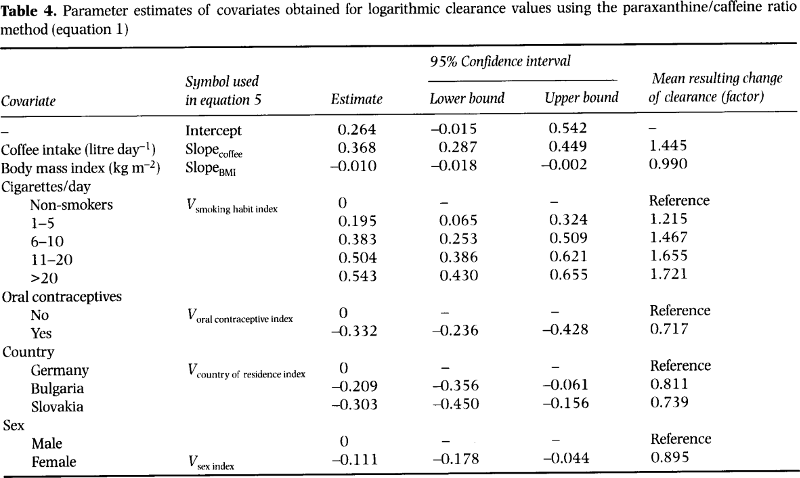
\includegraphics{figures/Tantcheva-Poor1999_Tab4.png}
\caption{Tab.1 Lifestyle Effects}
\end{figure}


    % Add a bibliography block to the postdoc
    
    
    
    \end{document}
